% ATENÇÃO - veja com o seu orientador se você vai ter este capítulo e se este vai ter nome!
\chapter{Metodologia}
\label{cap:metodologia}
Neste capítulo serão discutidos quais foram os passos já tomados e quais serão os passos para a elaboração deste trabalho, desde as pesquisas realizadas para o material bibliográfico, bem como um planejamento das futuras etapas, como pode ser observado na figura \ref{fig:metodologia:etapas} representando as etapas do trabalho. 

\begin{figure}[H]
    \centering
    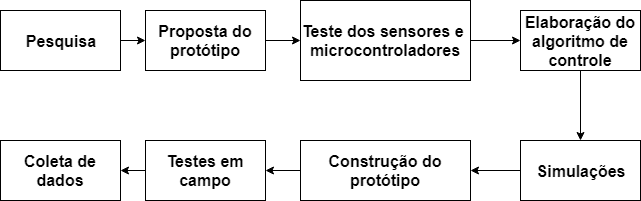
\includegraphics[width=0.8\textwidth]{figuras/metodologia.png}
    \caption{Fluxograma de etapas}
    \label{fig:metodologia:etapas}
\end{figure}

Com o tema definido, foram pesquisados artigos relacionados ao projeto de sistemas fotovoltaicos, o êxodo rural brasileiro, a mecanização do campo e agricultura de precisão, bem como trabalhos científicos com temáticas relacionadas a automação do  maquinário, da construção de protótipos, técnicas utilizadas em relação a movimentação dos veículos. A seguir, foram idealizados os componentes, bem como o chassi do veículo proposto. Durante a busca por trabalhos relacionados, foram usadas diversas bases de dados, tais como  \textit{Institute of Electrical and Electronics Engineers(IEEE) Xplore\footnote{https://ieeexplore.ieee.org/Xplore/home.jsp}, Google Scholar\footnote{https://scholar.google.com.br/},Sistema de Información Científica Redalyc 
Red de Revistas Científicas de América Latina y el Caribe\footnote{http://www.redalyc.org/home.oa}}, dentre outros bancos. 

A elaboração do protótipo foi feita em base das características de conceitos já testados em trabalhos relacionados. A adição do sistema fotovoltaico é um diferencial do projeto, já que a maioria utilizava apenas baterias ou motores a combustão. Com o avanço da pesquisa, serão realizadas revisões constantes no projeto do veículo a fim de aprimoro-lo e simplificar sua construção, viabilizando constantes aumentos de performance. 

Na fase do teste dos sensores e microcontroladores, serão testados quanto a funcionamento e compatibilidade, tendo em vista a simplicidade do projeto e o consumo energético para que posteriormente, sejam avaliados os requisitos do sistema fotovoltaico. Os  sensores serão avaliados quanto ao desempenho obtido, bem como a integração com as demais partes do sistema. Quanto aos microcontroladores, serão avaliados quanto ao desempenho de processamento dos dados dos sensores e atuadores a eles atrelados, bem como o funcionamento em conjunto e a viabilidade da utilização dos mesmos em um ambiente externo.

Quanto a elaboração do algoritmo do controle, está intimamente atrelada a fase anterior, já que a mesma baseia-se nos dados provenientes dos sensores utilizados. O mesmo deve ser elaborado utilizando a linguagem C/C++ compatível com o Arduino. Como exposto no capítulo \ref{cap:proposta}, o algoritmo a ser construído deve receber as informações dos \textit{N} sensores, combinar os dados dos mapas georreferenciados e ser capaz de controlar o veículo de forma precisa e segura, evitando obstáculos e corrigindo seu curso de momentos em momentos. Logo após as primeiras versões do algoritmo, simulações devem ser feitas com o objetivo de \textit{tunar}\footnote{Introduzir alterações e aprimoramentos em (carros, motocicletas, equipamentos eletroeletrônicos etc.), com o fito de personalizá-los ou melhorar o seu aspecto, desempenho etc.} os parâmetros, as estruturas de decisão e desempenho do sistema em geral. As simulações serão realizadas em ambiente controlado com objetivo de aferir o funcionamento do hardware e do software embarcado nesse sistema. Em paralelo a fase de simulação e elaboração o algoritmo, a construção odo veículo deve acontecer, visando a acomodação do sistema energético, os sensores e os atuadores. A construção deve ser ao mesmo tempo simples e robusta, dando condições a continuas mudanças de projeto.

Por fim, o teste em campo deve ser realizado afim de aferir e coletar os dados provenientes dos sensores para embasar a avaliação de desempenho do projeto como um todo. Ao fim dessa etapa será possível concluir se o projeto como todo é factível e viável, tendo sido feita uma avaliação da coleta de dados, medindo o desempenho do sistema fotovoltaico como solução  energética, a precisão dos trajetos e o recalculo do mesmo.
\newpage
Como esse projeto apresenta-se de forma relativamente ambiciosa, o mesmo deve obedecer um cronograma a altura, a fim de garantir a conclusão do mesmo, como pode ser observado na tabela \ref{cap:metodologia:cronograma} abaixo:
\begin{table}[h]
\centering
\caption{Cronograma}
\label{cap:metodologia:cronograma}
\begin{tabular}{|l|l|l|l|l|l|l|l|l|}
\hline
\multicolumn{1}{|c|}{}                             & \multicolumn{4}{c|}{\textbf{2018}}                                                                                                                      & \multicolumn{4}{c|}{\textbf{2019}}                                                                                                                      \\ \cline{2-9} 
\multicolumn{1}{|c|}{\multirow{-2}{*}{Atividades}} & \textbf{Ago}             & \textbf{Set}                                    & \textbf{Out}             & \textbf{Nov}                                    & \textbf{Jan}             & \textbf{Mar}                                    & \textbf{Maio}                                   & \textbf{Jun}             \\ \hline
Pesquisa                                           & \cellcolor[HTML]{000000} & \cellcolor[HTML]{000000}{\color[HTML]{000000} } & \cellcolor[HTML]{FFFFFF} &                                                 &                          &                                                 &                                                 &                          \\ \hline
Proposta do protótipo                              &                          &                                                 & \cellcolor[HTML]{000000} & \cellcolor[HTML]{000000}{\color[HTML]{000000} } &                          &                                                 &                                                 &                          \\ \hline
Testes dos sensores e microcontroladores           &                          &                                                 &                          &                                                 & \cellcolor[HTML]{000000} & \cellcolor[HTML]{FFFFFF}{\color[HTML]{000000} } &                                                 &                          \\ \hline
Elaboração do algoritmo de controle                &                          &                                                 &                          &                                                 & \cellcolor[HTML]{000000} & \cellcolor[HTML]{000000}{\color[HTML]{000000} } & {\color[HTML]{000000} }                         &                          \\ \hline
Simulações                                         &                          &                                                 &                          &                                                 &                          & \cellcolor[HTML]{000000}{\color[HTML]{000000} } &                                                 &                          \\ \hline
Construção do protótipo                            &                          &                                                 &                          &                                                 &                          & \cellcolor[HTML]{000000}{\color[HTML]{000000} } & \cellcolor[HTML]{000000}{\color[HTML]{000000} } &                          \\ \hline
Teste em campo                                     &                          &                                                 &                          &                                                 &                          &                                                 & \cellcolor[HTML]{000000}{\color[HTML]{000000} } &                          \\ \hline
Coleta de dados                                    &                          &                                                 &                          &                                                 &                          &                                                 &                                                 & \cellcolor[HTML]{000000} \\ \hline
\end{tabular}
\end{table}
